%! TEX root = ../../main.tex

\subsection{Helm}%
\label{sub:Helm}
Up to this point, users who wanted to deploy their application to Kubernetes
always had to define their application's Kubernetes manifests and then apply them
manually e.g.\ by using the \texttt{kubectl} utility. This approach however
lacks the important ability to define dependencies. Thus, a microservice
architecture that consists of microservice $A$ which internally requires
microservice $B$ so be installed as well is hard to set up. Should both
microservices be defined in the same manifest file? This would reduce
reusability. Should they be split into two manifests? Should they be stored in
the same directory? This would again reduce the reusability but ease the
deployment of both services because the full folder could be applied to the
Kubernetes cluster. One might say that such a problem is already solved for the
development of applications in many languages. When using JavaScript with
Node.js, the \ac{NPM} utility can manage the dependencies of a project.
Additionally it not only installs them but manages their complete lifecycle
\autocite{npm}. With the help of a one command \texttt{npm install
\textbf{my-app} -g} \ac{NPM} takes care of installing the full application
without demanding any further input from the user.

This functionality however seems fairly absent from Kubernetes. This is where
the \textit{Helm} project has to be introduced. Helm acts as a package manager
for Kubernetes. It consists of two components. The first component is the
\textit{Helm} client which runs on the user's computer and \textit{Tiller}
which runs inside the Kubernetes cluster. Tiller's job is to manage the
Kubernetes objects that the Helm client want to deploy to the cluster. Instead
of running Helm on a developer's local machine, it is also possible to execute
it as part of \ac{CI}/\ac{CD} pipeline \autocite{HelmDocumentationQuickstart}.
The possibilities of \ac{CI}/\ac{CD} pipelines will be further discussed in the
upcoming chapter~\ref{sub:Automatic_a_Microservices_Deployment}.

Helm imposes a strict file structure upon projects that use it. Like the
Kubernetes utility \texttt{kubectl}, Helm configurations are defined in YAML
files. A set of configurations for an application is called \textit{chart}.
Each chart is stored in a distinct directory which is named after the chart.
Thus, when e.g.\ defining a chart called \textit{documentation-service}, the
directory holding all the application's Helm configurations is also called
\texttt{documentation-service}. 

\begin{figure}[H]
\begin{center}
  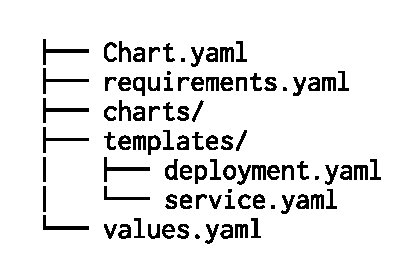
\includegraphics[scale=0.8]{images/figures/directory_listing_example_chart.pdf}
\end{center}
\caption{Visualised folder structure of an exemplary Helm chart.}%
\label{fig:helm_chart_folder_example}
\end{figure}

Figure~\ref{fig:helm_chart_folder_example} shows a set of Helm configurations
that are commonly used. The only mandatory file however is the
\texttt{Charts.yaml}. It holds the chart's basic settings like name, author(s)
and version number. The \texttt{requirements.yaml} file stores references to
other charts that Helm can download into the \texttt{charts/} directory before
deploying a chart. Theses charts are also known as \textit{sub-charts}. A
backend e.g.\ would reference a \textit{Neo4j} graph database. Every time this
backend is deployed to Kubernetes, Helm would make sure to also deploy the
referenced Neo4j database sub-chart. Once an application is deployed by Helm,
it is referred to as being a \textit{release}. Releases can be upgraded to new
versions or even rolled back to a previously deployed version. Besides that,
the \texttt{templates/} directory holds actual Kubernetes manifests. Thus, to
\textit{helmify} an application that needs to define a Kubernetes Service and
Deployment, the templates directory can hold two files describing these
objects. The power of defining and managing dependencies might already enhance
a basic deployment process drastically tough Helm's power lays in its
templating ability. The Kubernetes manifests inside the templates directory may
also include dynamic values. These values can either be provided by Helm
directly, like the release's name, or set by the user inside the
\texttt{values.yaml} file. In addition, values can also be set for sub-charts
\autocite{HelmDocumentationCharts}. The way these Helm configurations have to
be structured will not be further explored in this section as the practical use
will become clear in the upcoming solution searching process. A full list of
properties and additional files can nonetheless be found at
\autocite{HelmDocumentationCharts}.

The last aspect of Helm that will be examined is the ability to share 
charts. Once a chart is fully defined, Helm can package all its files into a
\texttt{tgz} archive. This archive can then be published to a public chart
repository, e.g.\ \textit{Helm Hub} which can be compared to \textit{Docker
Hub}, or a private one. When a chart is published to a repository, users can
fetch it and install it as if the chart would be written on their local
machine \autocite{HelmDocumentationCharts}. With this functionality Helm brings
the comfort known from package managers like \ac{NPM} or Docker to Kubernetes.
